% Setup
\documentclass[12pt]{article}
\title{\vspace{-60pt}MATH38161 Multivariate Statistics and Machine Learning Coursework}
\author{Name: Josh Mottley}
\date{\today}

% Packages
\usepackage{geometry}
\usepackage{lingmacros}
\usepackage{amsmath}
\usepackage{siunitx}
\usepackage{graphicx}
\usepackage[svgnames]{xcolor}
\usepackage{listings}
\usepackage{csquotes}
\usepackage{float}

%Slightly bigger size: \scriptsize
\lstset{
  language=R,                     % the language of the code
  basicstyle=\scriptsize\ttfamily, % the size of the fonts that are used for the code
  numbers=left,                   % where to put the line-numbers
  numberstyle=\scriptsize\color{Blue},  % the style that is used for the line-numbers
  stepnumber=1,                   % the step between two line-numbers. If it is 1, each line
                                  % will be numbered
  numbersep=5pt,                  % how far the line-numbers are from the code
  backgroundcolor=\color{white},  % choose the background color. You must add \usepackage{color}
  showspaces=false,               % show spaces adding particular underscores
  showstringspaces=false,         % underline spaces within strings
  showtabs=false,                 % show tabs within strings adding particular underscores
  frame=single,                   % adds a frame around the code
  rulecolor=\color{black},        % if not set, the frame-color may be changed on line-breaks within not-black text (e.g. commens (green here))
  tabsize=2,                      % sets default tabsize to 2 spaces
  captionpos=t,                   % sets the caption-position to bottom
  breaklines=true,                % sets automatic line breaking
  breakatwhitespace=false,        % sets if automatic breaks should only happen at whitespace
  deletekeywords={data,frame,length,as,character},
  keywordstyle=\color{RoyalBlue},      % keyword style
  otherkeywords={},
  commentstyle=\color{DarkGreen},   % comment style
  stringstyle=\color{ForestGreen}      % string literal style
}

\lstset{literate=%
   *{0}{{{\color{RoyalBlue}0}}}1
    {1}{{{\color{RoyalBlue}1}}}1
    {2}{{{\color{RoyalBlue}2}}}1
    {3}{{{\color{RoyalBlue}3}}}1
    {4}{{{\color{RoyalBlue}4}}}1
    {5}{{{\color{RoyalBlue}5}}}1
    {6}{{{\color{RoyalBlue}6}}}1
    {7}{{{\color{RoyalBlue}7}}}1
    {8}{{{\color{RoyalBlue}8}}}1
    {9}{{{\color{RoyalBlue}9}}}1
    {TRUE}{{{\color{RoyalBlue}TRUE}}}4
    {FALSE}{{{\color{RoyalBlue}FALSE}}}5
    {<-}{{{\color{Gray}<-}}}2
}

% Commands/Setup
\newcommand{\vect}[1]{\boldsymbol{#1}}
\newcommand{\mat}[1]{\underline{\boldsymbol{#1}}}
\newcommand{\mean}[1]{\bar{#1}}
\newcommand{\trans}[1]{#1^T}
\newcommand{\est}[1]{\hat{#1}}
\renewcommand{\exp}[1]{\text{exp}\left(#1\right)}

\geometry{
a4paper,
left=15mm,
top=20mm,
bottom=20mm,
right=15mm,
heightrounded
}
\setlength{\parindent}{0em}
\setlength{\parskip}{1em}

\graphicspath{{./Images/}}

% Document
\begin{document}

% Title page
\maketitle

\section*{Introduction}
For this report I will be using bold letters to represents vectors (e.g: $\vect{A}$), bold and underlined letters to show matrices (e.g: $\mat{B}$). A full example may look like:
\begin{equation*}
\vect{y}=\vect{\beta}\mat{X}
\end{equation*} \par

Futhermore, note that the "Appendix" chapter does not need to be viewed, and only contains the whole code, including testings, written, and should only be viewed if futher detail is needed.

% Start
\section{One-dimensional Gaussian mixture model and the inference with the EM algorithm}
The analytical update formula in the EM algorithm, for estimation of the parameters of a K-component mixture of one-dimensional normal distribution, can be written down as the E (expectation) and M (Maximisation) step equations.
\subsection{Expectation step}
The E "expectation" step of the EM algorithm is given by using Bayes theorem to predict the probabilities of allocations for all samples $x_i$, i.e:
\begin{equation} \label{Def:Exp}
  \mat{z}_{ik}^{(b+1)} = \frac{\vect{\pi}_kF(\vect{x}_i|\vect{\theta}_k)} {\sum_{j=1}^K[\vect{\pi}_jF(\vect{x}_i|\vect{\theta}_j)]}
\end{equation}
where $\vect{\pi}$ is the weights of each group of $\mat{z}_{ik}^{(b)}$, $F$ is the probability density function, $K$ is the number of assumed groups, $\vect{\theta}^{(b)}$ is the current parameter vector for each group k, $\vect{x}$ is the observed data, and $\mat{z}_{ik}^{(b)}$ is the current probability distribution of the latent variable $k$.

First of, to calculate the weights $\vect{\pi}_k$ of each group of $\mat{z}_{ik}^{(b)}$, we use:
\begin{equation*}
  \vect{\pi}_k=\frac{\sum_{i=1}^n\mat{z}_{ik}^{(b)}}{n}
\end{equation*}

So now calculate the E step for 1-dimensional Gaussian mixture models using (\ref{Def:Exp}):
\begin{align} \label{Gau:Exp}
  \mat{z}_{ik}^{(b+1)} & = \frac{\vect{\pi}_kF(\vect{x}_i|\vect{\mu}_k, \vect{\sigma^2}_k)}
                                {\sum_{j=1}^K[\vect{\pi}_jF(\vect{x}_i|\vect{\mu}_j, \vect{\sigma^2}_j)]} \nonumber
                           \\
                       & = \frac{\vect{\pi}_k\left(\frac{1}{\sqrt{2\pi\vect{\sigma}_k^2}}\right)
                                  \exp{-\frac{(\vect{x}_i-\vect{\mu}_k)^2} {2\vect{\sigma}_k^2}}}
                                {\sum_{j=1}^K\vect{\pi}_j\left(\frac{1}{\sqrt{2\pi\vect{\sigma}_j^2}}\right)
                                  \exp{-\frac{(\vect{x}_i-\vect{\mu}_j)^2} {2\vect{\sigma}_j^2}}}
\end{align}
where $\mu$ is the mean vector, and $\sigma^2$ is the variance vector.

\subsection{Maximisation step}
The maximisation step involves computing the expected complete data log-likelihood function using the new weights, and then maximising the function to update the mixture model parameter $\vect{\theta}$, which will be the maximum likelihood parameter. This can be also be described by the following equations
\begin{gather}
  \label{Gau:Max:Func}
  Q(\vect{\theta}|\vect{\theta}^{(b)}) =
          \sum_{i=1}^n\sum_{k=1}^K\mat{z}_{ik}^{(b+1)}\log(\vect{\pi}_kF_k(\vect{x}_i)) \\
  \label{Gau:Max:Max}
  \vect{\theta}^{(b+1)} \leftarrow \arg\max_{\vect{\theta}}Q(\vect{\theta}|\vect{\theta}^{(b)})
\end{gather}
First we want to find the complete log-likelihood part in (\ref{Gau:Max:Func}), which is given by:
\begin{align} \label{Gau:Max:Likelihood}
  l(\vect{\mu}, \vect{\sigma}|\vect{x}_i)
                  & = \sum_{i=1}^n\sum_{k=1}^K\log(\vect{\pi}_kF_k(\vect{x}_i)) \nonumber \\
          & = \sum_{i=1}^n\sum_{k=1}^K\left[\log{\vect{\pi}_k-\frac{1}{2}\log2\pi-\frac{1}{2}\log\vect{\sigma}^2_k}
                                    -\frac{1}{{2\sigma^2}}(\vect{x}_i-\vect{\mu}_k)^2\right]
\end{align}
Now we want to find $Q$, by substituting (\ref{Gau:Max:Likelihood}) into (\ref{Gau:Max:Func}) to get:
\begin{equation} \label{Gau:Max:Q}
  Q(\vect{\theta}|\vect{\theta}^{(b)}) =  \sum_{i=1}^n\sum_{k=1}^K
            \mat{z}_{ik}^{(b+1)}\left[\log{\vect{\pi}_k-\frac{1}{2}\log2\pi
            -\frac{1}{2}\log\vect{\sigma}^2_k}-\frac{1}{{2\sigma^2}}(\vect{x}_i-\vect{\mu}_k)^2\right]
\end{equation}
Subbing (\ref{Gau:Max:Q}) into (\ref{Gau:Max:Max}) for 1-dimensional Gaussian, we get:
\begin{equation} \label{Gau:Max:Para}
  (\vect{\mu}_k^{(b+1)}, \vect{\sigma}_k^{(b+1)})
              = \arg\max_{\vect{\mu}_k, \vect{\sigma}_k} \sum_{i=1}^n
                        \mat{z}_{ik}^{(b+1)}\left[\log{\vect{\pi}_k-\frac{1}{2}\log2\pi
                        -\frac{1}{2}\log\vect{\sigma}^2_k}-\frac{1}{{2\sigma^2}}(\vect{x}_i-\vect{\mu}_k)^2\right]
\end{equation}
Take the derivatives $\vect{\mu}$ and $\vect{\sigma}^2$ of (\ref{Gau:Max:Para}), and set each to 0 and solve, leading to the predicition of the next parameters as:
\begin{gather}
  \vect{\mu}_k^{(b+1)}=\frac{\sum_{i=1}^n\mat{z}_{ik}^{(b)}\vect{x}_i}{\sum_{i=1}^n\mat{z}_{ik}} \\
  \vect{\sigma}_k^{(b+1)}=\frac{\sum_{i=1}^n\mat{z}_{ik}^{(b)}(\vect{x}_i-\vect{\mu}_k^{(b)})^2}
                               {\sum_{i=1}^n\mat{z}_{ik}}
\end{gather}

\section{Implementation of 1-dimensional gaussian EM algorithm with R}
For the full code regarding the implementation (i.e the function and testing), refer to Listing-\ref{R_complete_code}.
\subsection{The EM function}
The R function that performs EM estimation and returns the model parameters, as well as the probabilities of each sample that belongs to one of the K classes for 1-dimensional gaussion is given by:
\UseRawInputEncoding
\begin{lstlisting}[caption={EM function}]
# EM algorithm function
# @param: x     : the data
# @param: K     : number of classes
# @param: it    : number of iterations
emAlgo<-function(x, K, it)
{
  # Initilise z_ik with a random soft allocation
  z_ik<-matrix(runif(K*length(x), 0, 1), ncol=K)
  # Normalise matrix (so sum of groups per sample = 1)
  correction<-z_ik[, 1]+ z_ik[, 2]
  z_ik[, 1]<-z_ik[, 1]/correction
  z_ik[, 2]<-z_ik[, 2]/correction
  # Initialise variables
  nk=0
  weights=0
  mean=0
  var=0
  # Iterate through the E and M steps
  for(iter in 1:it)
  {
    # Perform the M-step
    nk=colSums(z_ik)
    weights=nk/length(x)
    mean=apply(z_ik, 2, `%*%`, x)/nk
    var=colSums(z_ik*(outer(x, mean, "-")^2))/nk
    # Perform the E-step
    normal.d=t(sapply(x, dnorm, mean=mean, sd=sqrt(var)))
    z_ik=apply(normal.d*weights[col(normal.d)], 2, "/", rowSums(normal.d*weights[col(normal.d)]))
  }
  # Store in data frame
  output<-list(
    "parameters"=cbind(mean, sd=sqrt(var)),
    "z_ik"=z_ik
    )

  # Return Output
  return(output)
}
\end{lstlisting}

\subsection{Analysis of data}
Now if we test this by applying the function with 10000 iterations (to try to get convergence) to the following vector of $n = 10$ observations with $K = 3$: \par
$x = c(4.54,1.57,1.41,1.77,1.43,0.07,0.05,4.19,−0.02,1.32)$ \par
Resulting in the following output:
\begin{lstlisting}[caption={Complete R code output},label={R_complete_output}]
> print(out$parameters)
           mean         sd
[1,] 1.50000000 0.15697133
[2,] 0.03333333 0.03858612
[3,] 4.36500000 0.17500000
> print(out$z_ik)
              [,1]          [,2]          [,3]
 [1,] 1.651920e-81  0.000000e+00  1.000000e+00
 [2,] 1.000000e+00  0.000000e+00  1.609491e-56
 [3,] 1.000000e+00 1.126038e-276  5.147652e-63
 [4,] 1.000000e+00  0.000000e+00  2.815409e-48
 [5,] 1.000000e+00 8.586318e-285  3.301200e-62
 [6,] 6.127144e-19  1.000000e+00 3.667272e-132
 [7,] 1.330678e-19  1.000000e+00 1.540945e-133
 [8,] 7.799149e-64  0.000000e+00  1.000000e+00
 [9,] 4.636914e-21  1.000000e+00 1.753860e-137
[10,] 1.000000e+00 1.677989e-241  1.249908e-66
\end{lstlisting}
Now look at the density graph of the data given ($x$):
\begin{figure}[H]
    \centering
    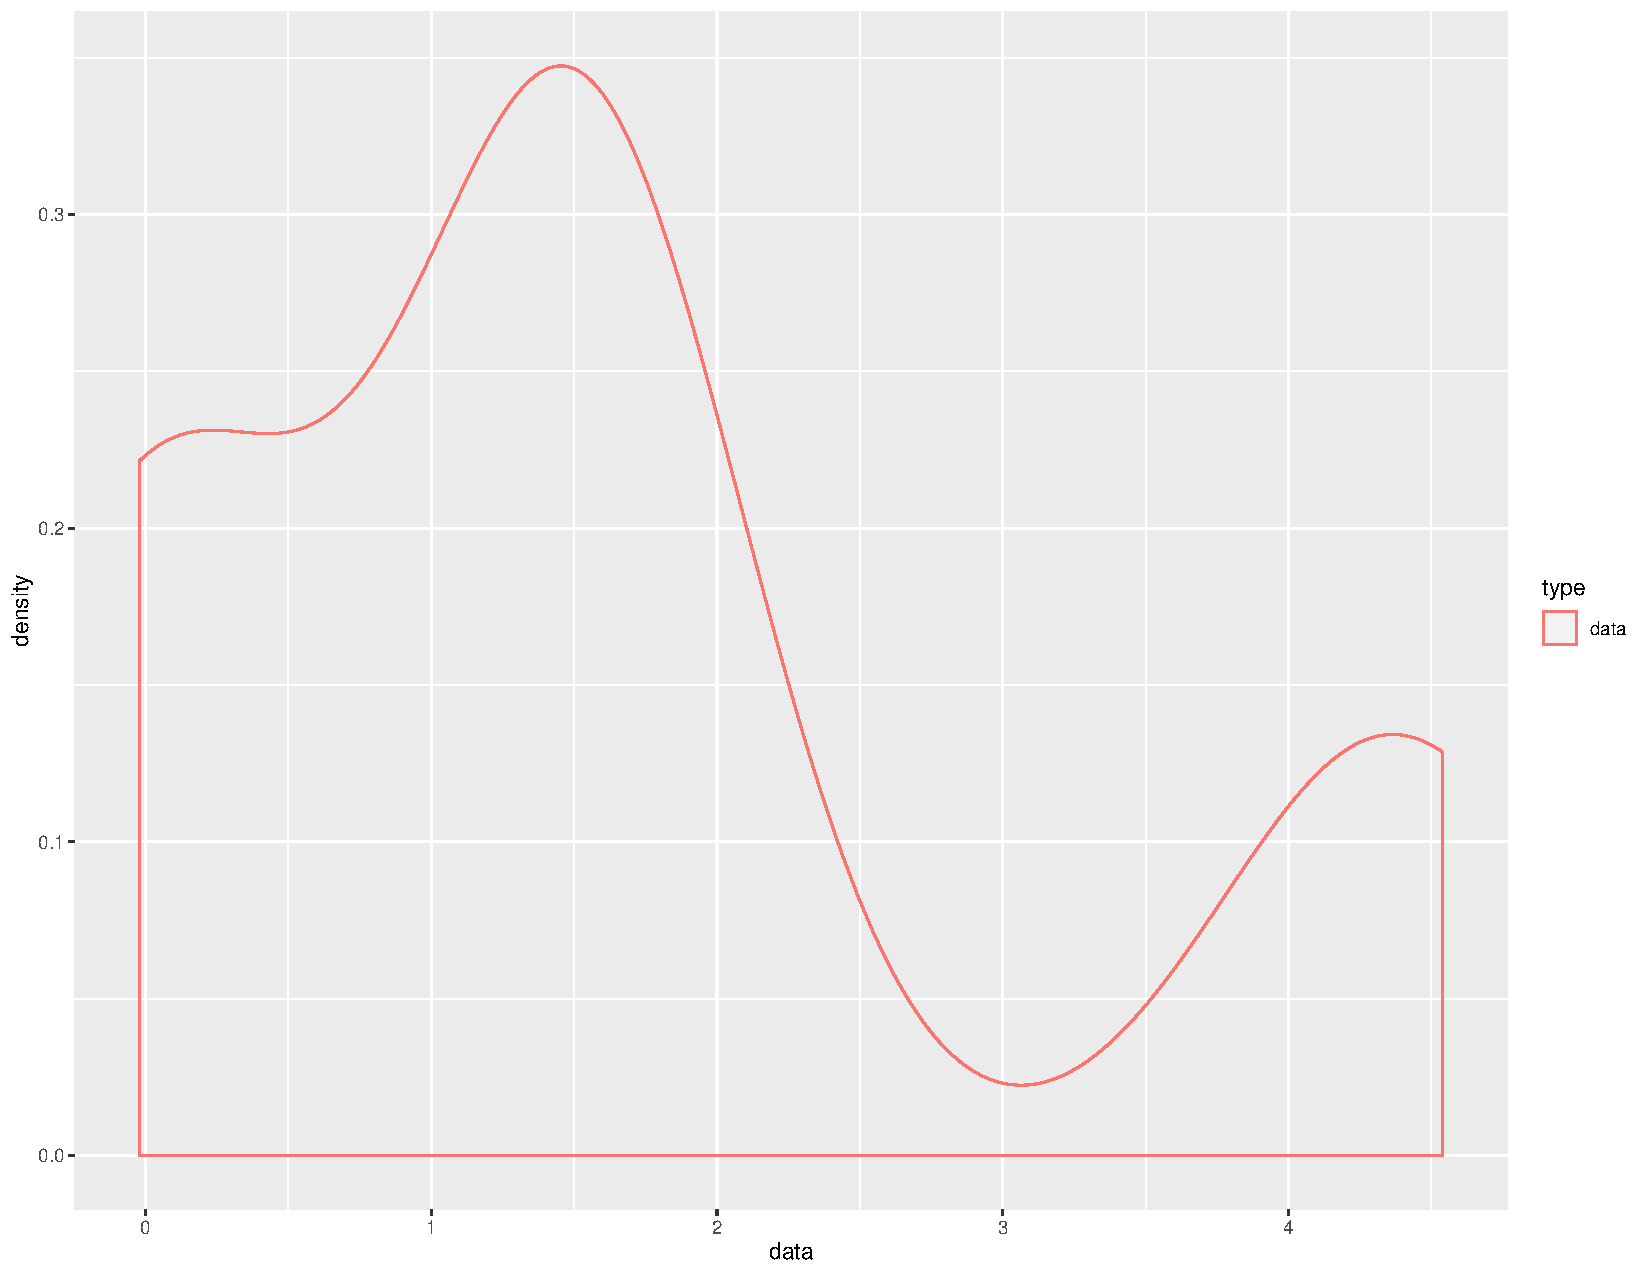
\includegraphics[width=\textwidth]{DensityGraph.pdf}
    \caption{Plot of density of example data}
\end{figure}
Using the assumption that there are 3 groups, we can see 3 Gaussian distributions, with rough means between $(0-1)$, $(1-2)$ and $(4-5)$. This aligns with the results of the parameters returned from the function at 0.03333333, 4.36500000, 1.50000000. Futhermore, we can see from the graph that the right data have a wider spread than the middle, which can also been seen by the standard deviation of the group with mean 4.36500000 being higher than the sd of the group with mean 1.50000000. Altogether, when comparing the graph of the data, against the results after testing the functions I can confidently say that the EM function is successful at determining the parameters of a mixed Gaussian model, with the downside being that it can take many iterations of the algorithm to successfully converge to the parameters.

\section{Appendix}
\UseRawInputEncoding
\begin{lstlisting}[caption={Complete R code (Function and testing)},label={R_complete_code}]
# Delete previous variables
rm(list=ls())
dev.off()

# Includes
library("ggplot2")

# EM algorithm function
# @param: x     : the data
# @param: K     : number of classes
# @param: it    : number of iterations
emAlgo<-function(x, K, it)
{
  # Initilise z_ik with a random soft allocation
  z_ik<-matrix(runif(K*length(x), 0, 1), ncol=K)
  # Normalise matrix (so sum of groups per sample = 1)
  correction<-z_ik[, 1]+ z_ik[, 2]
  z_ik[, 1]<-z_ik[, 1]/correction
  z_ik[, 2]<-z_ik[, 2]/correction
  # Initialise variables
  nk=0
  weights=0
  mean=0
  var=0
  # Iterate through the E and M steps
  for(iter in 1:it)
  {
    # Perform the M-step
    nk=colSums(z_ik)
    weights=nk/length(x)
    mean=apply(z_ik, 2, `%*%`, x)/nk
    var=colSums(z_ik*(outer(x, mean, "-")^2))/nk
    # Perform the E-step
    normal.d=t(sapply(x, dnorm, mean=mean, sd=sqrt(var)))
    z_ik=apply(normal.d*weights[col(normal.d)], 2, "/", rowSums(normal.d*weights[col(normal.d)]))
  }
  # Store in data frame
  output<-list(
    "parameters"=cbind(mean, sd=sqrt(var)),
    "z_ik"=z_ik
    )

  # Return Output
  return(output)
}

###########################################################
# Test function
###########################################################

# Create data
x = c(4.54,1.57,1.41,1.77,1.43,0.07,0.05,4.19,-0.02,1.32)
y = factor(c(rep("data", length(x))))

# Plot data
df <- data.frame(
  type=y,
  data=x
)
ggplot(df, aes(x=data, color=type)) +
  geom_density()

# Test function
out<-emAlgo(x, 3, 10000)

# Output possible values
print(out$parameters)
print(out$z_ik)
\end{lstlisting}

\end{document}
